\documentclass[12pt]{article}

\usepackage{graphicx,color,enumerate,multicol}
\usepackage[top=1in, bottom=1in, left=1.25in, right=1.25in]{geometry}
\usepackage{tikz,pgfplots}

%% Use Minion fonts if available.  Otherwise Times.
\IfFileExists{MinionPro.sty}{\usepackage[lf]{MinionPro}}{}
\usepackage{amsmath,amsthm,amsbsy}
\IfFileExists{MinionPro.sty}{}{\usepackage{times,txfonts}}

%% Setup aproblem environment, 
%% aproblem items
%% subproblems environment
%% subproblem items
\makeatletter
\newcounter{probcount}
\newcounter{subprobcount}
\newlength\probsep
\newlength\pshrinking
\newif\iffirstprob
\newenvironment{aproblems}%
  {\ifhmode\unskip\par\fi\setcounter{probcount}{0}\probsep\parskip
  \sbox\@tempboxa{\textbf{9.}}\pshrinking\wd\@tempboxa\advance\pshrinking\labelsep
  \let\hproblem\aproblem
  \advance\linewidth -\pshrinking
  \advance\@totalleftmargin\pshrinking
  \advance\leftskip\pshrinking}%
  {\ifhmode\unskip \par\fi\advance\leftskip-\pshrinking}%

\newcommand{\aproblem}{%
  \setcounter{subprobcount}{0}%
  \stepcounter{probcount}%
  \def\@currentlabel{\arabic{probcount}}%
  \ifhmode
    \unskip \par
  \fi
%  \addpenalty{-4000}%
  \iffirstprob\else\addvspace\probsep\fi
  \firstprobfalse
  \hskip -\labelwidth\hskip -\labelsep 
  \hbox to\labelwidth{\hss\textbf{\arabic{probcount}.}}\hskip\labelsep
}%

\newcommand{\subprob}{\item\def\@currentlabel{\arabic{probcount}\alph{\thelistlabel}}}
\newcommand{\skipproblem}{\stepcounter{probcount}}


%% The following commands put defined left and right headers on the top, and a page number
%% on the bottom of all pages beyond page 1
\usepackage{fancyhdr}
\pagestyle{fancy}
\fancyfoot[C]{\ifnum \value{page} > 1\relax\thepage\fi}
\fancyhead[L]{\ifx\@doclabel\@empty\else\@doclabel\fi}
\fancyhead[R]{\ifx\@docdate\@empty\else\@docdate\fi}
\headheight 15pt
\def\doclabel#1{\gdef\@doclabel{#1}}
\def\docdate#1{\gdef\@docdate{#1}}
\makeatother

%% General formatting parameters
\parindent 0pt
\parskip 6pt plus 1pt

\let\ds\displaystyle
\doclabel{Math F251X: Midterm 1 Review}
\docdate{24 September 2019}


\begin{document}
\begin{aproblems}

\aproblem State the definition of the derivative of a function $f(x)$ at $x=a$.
\vspace{1in}

\aproblem Let $f(x)=5x^2-3x$.
\renewcommand{\labelenumi}{\textbf{(\alph{enumi})}}
\begin{enumerate}
\item Use the definition to find the derivative of $f(x).$ 
\vspace{3in}
\item Find the slope of the tangent line to $f(x)$ when $x=-3.$
\vfill
\item Write the equation of the line tangent to $f(x)$ when $x=-3.$
\vfill
\end{enumerate}

\newpage

\aproblem Suppose $N$ represents the number of people in the United States who travel by car to another state for a vacation this Memorial Day weekend when the average price of gasoline is $p$ dollars per gallon. 
\begin{enumerate}
\item What are the units of $dN/dp$?\\
\item In the context of the problem, write a sentence interpreting $\frac{dN}{dp}.$\\
\vspace{0.5in}
\item Would you expect $dN/dp$ to be positive or negative? Explain your answer.
\vfill
\end{enumerate}

\aproblem The graph of $f(x)$ is sketched below. On a separate set of axes, give a rough sketch $f'(x).$\\

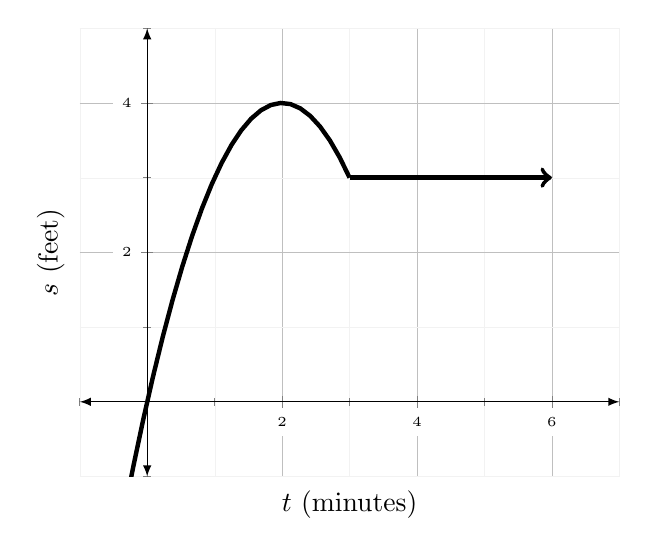
\begin{tikzpicture}[scale=1]
\begin{axis}[grid style={line width=.1pt, draw=gray!10},grid=both,major grid style={line width=.2pt,draw=gray!50},
    xmin=-1,xmax=7,
    ymin=-1,ymax=5,
    xtick={},ytick={},
    minor tick num=1,
    enlargelimits={abs=0},
    ticklabel style={font=\tiny,fill=white},
    axis lines=middle,
    axis line style={latex-latex},
    x label style={at={(axis description cs:0.5,-0.01)},anchor=north},
    y label style={at={(axis description cs:-0.01,.5)},rotate=90,anchor=south},
        xlabel={$t$ (minutes)},
    ylabel={$s$ (feet)}
]
\addplot[<-,domain=-0.5:3,ultra thick] {-(x-2)^2+4};
\addplot[->,domain=3:6,ultra thick] {3};
\end{axis}
\end{tikzpicture}

\aproblem Find the domain of each function.
\begin{multicols}{2}
\begin{enumerate}
\item $f(x)=\sqrt{x^2-x-6}$

\item $g(t)= \ln (t+6)$

\end{enumerate}
\end{multicols}
\vfill

\newpage

\aproblem State the definition of ``The function $f(x)$ is continuous at $x=a$''.
\vskip 1in

\aproblem Suppose
$$
f(x) = \begin{cases} -\frac{2}{x} & x < 2\\
\frac{x}{x-3} & x \ge 2\end{cases}
$$
Is $f(x)$ continuous at $x=0$?  At $x=2$? Justify your answers
using the definition of continuity.
\vfill

\aproblem Find the limit or show that it does not exist. \emph{Make sure you are writing your mathematics correctly and clearly.}
\begin{enumerate}
\item $\ds{\lim_{x \to \infty} \frac{10^x-1}{3-10^x}}$\\
\vfill
\item $\ds{\lim_{x \to \infty} \frac{\sqrt[3]{8x^3+1}}{2-5x}}$\\
\vfill
\item $\ds{\lim_{r \to 16^-} \frac{\sqrt{r}}{(r-16)^3}}$\\
\vfill
\item $\ds{\lim_{x \to -3} \frac{x^2-9}{x^2+2x-3}}$\\
\vfill
\end{enumerate}

\newpage

\aproblem Consider a function with vertical asymptotes at $x=-1$ and $x=3$ and a horizontal asymptote at $y=4/3.$

\begin{enumerate}
\item Write a formula for such a function.
\vfill

\item Sketch the graph of the function.
\vfill
\item Use limits to demonstrate that your function really does have a vertical asymptote at $x=-1$
\vfill

\item Use limits to demonstrate that your function really does have a horizontal asymptote at $y=4/3.$
\vfill
\end{enumerate}

\aproblem Solve for $x.$
\begin{multicols}{2}
\begin{enumerate}
\item $e^{x-3}+2=6$\\
\vspace{1in}
\item $\ln(x+5)-3=7$
\columnbreak
\item $\ln x + \ln (x-1) =0$
\vspace{1in}
\item $\cos(8x)=0$
\end{enumerate}
\end{multicols}
\vfill

\newpage
\aproblem Use the Intermediate Value Theorem to show $\ln x = x-5$ has a solution. (Hint: Show there is a solution in the interval $[1,e^5].$)
\vspace{2in}

\aproblem Sketch each of the functions below. Label all $x$- and $y$-intercepts and asymptotes. State, in interval notation, the domain and range of each function next to its graph.\\
\begin{multicols}{3}
\begin{enumerate}
\item $y=6-x^4$
\item $y=\sin(2x)$
\item $y=\tan x$
\item $y=\tan^{-1} x$
\item $y=e^{x-1}+2$
\item $y=\ln x$
\item $y=-2/(x+3)$
\item $y=\sqrt{x+5}$\\
\quad
\end{enumerate}
\end{multicols}

\end{aproblems}

\end{document}